% Generated from ../writeup.md by md2tex.py. Every number comes from ../../results/summary.md
% and ../../results/summary_replays.md. Build: tectonic ooda_aegis.tex (or pdflatex twice).
\documentclass[10pt,a4paper]{article}
\usepackage[T1]{fontenc}
\usepackage[utf8]{inputenc}
\usepackage{lmodern}
\usepackage{microtype}
\usepackage[margin=2.2cm]{geometry}
\usepackage{amsmath,amssymb}
\usepackage{booktabs}
\usepackage{graphicx}
\usepackage{enumitem}
\usepackage{xcolor}
\usepackage[hidelinks]{hyperref}
\usepackage{titlesec}
\usepackage{adjustbox}
\usepackage{float}
\setlength{\tabcolsep}{4.5pt}
\setlength{\emergencystretch}{2em}
\setlist{nosep,leftmargin=*}
\titlespacing*{\section}{0pt}{1.2ex plus .4ex}{0.6ex}
\titlespacing*{\subsection}{0pt}{1.0ex plus .3ex}{0.4ex}
\setlength{\parskip}{0.45ex}
\newcommand{\phisafe}{\ensuremath{\Phi_{\mathrm{safety}}}}

\title{\textbf{OODA-Aegis:\\Exploit-Grounded, Constraint-Verified Program Repair with Gemma 4}\\[0.6ex]\large A Gemma 4 agent that finds exploited code through the call graph, proves its actions safe with Z3, and verifies every fix.}
\author{Nikhil Kumar (lead author) \and Suryansh Pratap Singh}
\date{\small Code, benchmark, raw logs and notebooks: \url{https://github.com/CopyNinja07-07/aegis}}
\begin{document}
\maketitle
\begin{abstract}
Small open models can write security patches, but their own tests cannot be trusted: the repair model's test agreed with an independent verifier on only 56\% of candidates. OODA-Aegis, an Observe-Orient-Decide-Act agent on Gemma 4, treats every model output as an untrusted proposal: it retrieves code through the call graph, has the Z3 SMT solver check every action, and accepts a patch only when an agent-built gate shows the exploit worked before and fails after, with legitimate traffic unchanged. On AegisBench (16 tasks, 9 vulnerability classes, free Kaggle T4 GPUs) the agent verified 45 of 48 fixes; the route file alone gave 0 of 32, trusting the model's own test shipped 4 broken patches, and E4B matched 31B at four times the speed. With bugs up to five call hops away, the call slice verified 27 of 32 fixes against 15 for the whole repository, while a 2-hop limit passed the gate only by guarding an outer layer, which a dynamic-taint clause rejects. On 13 real CVEs with reproducing exploits (up to 151k lines), graph plus exploit trace reaches every bug and works best as a filter for similarity ranking; on CVE-2021-33503 the verified patches were mitigations, not the upstream fix. Simple injections never changed the model's actions.

\end{abstract}
\section{Introduction}
Coding agents are judged by whether a patch makes tests pass; for security fixes this is too weak (a variant of the attack can still work) and circular (the model that wrote the patch often wrote the test). The agent's actions can also do harm, and attackers reach its context through the traffic it analyses.

Following Boyd's loop~\cite{r14}, we cast this as a constrained POMDP~\cite{r15}: hidden state is the code and the attacker's capability; observations are responses, timings and redirects; actions are an edge rule $a_{\mathrm{edge}}$ and a patch $a_{\mathrm{patch}}$, constrained by a safety predicate \phisafe{}. The model proposes $a \sim \pi_\theta(\cdot \mid \text{evidence}, \text{context})$; the agent executes the projection

\begin{equation}
a_{\mathrm{exec}} =
\begin{cases}
a & \text{if Z3 proves } \phisafe(a),\\
\text{conservative fallback (no rule, no patch, escalate)} & \text{otherwise.}
\end{cases}
\end{equation}
\textbf{Contributions.} (1) \textbf{AegisBench}, 16 executable repair tasks with outcome oracles, held-out variants and legitimate-traffic checks, and \textbf{AegisBench-Deep}, which moves each bug up to five call hops away. (2) \textbf{OODA-Aegis on Gemma 4}: exploit grounding, code-graph retrieval, Z3-checked actions, multi-candidate search and an agent-built gate. (3) Retrieval across dynamic, decorator and ORM indirection and 13 real CVEs with exploits and regression tests, two data-flow clauses, and the full loop on one real CVE.

\textbf{Findings.} (F1) Localisation is the bottleneck: the same model goes from 0/32 to 45/48 when it sees the files the call graph selects, 7\% of the code; with the bug out of view it passes the gate only by guarding an outer layer. (F2) Model-written tests are a weak acceptance signal. (F3) Inside a verifying loop, the 4B-effective model is as reliable as 31B. (F4) Retries mostly paid for one formatting error. (F5) Simple, static injections did not move Gemma 4; adaptive attacks are untested.

\textbf{Track topics.} \emph{Code Comprehension} (\S{}2, \S{}4.2, \S{}4.3), \emph{Tasks \& Benchmarks} (\S{}3), data for \emph{Tuning \& Optimization} (\S{}6), an application (\S{}5).

\section{Methods}
\begin{figure}[H]\centering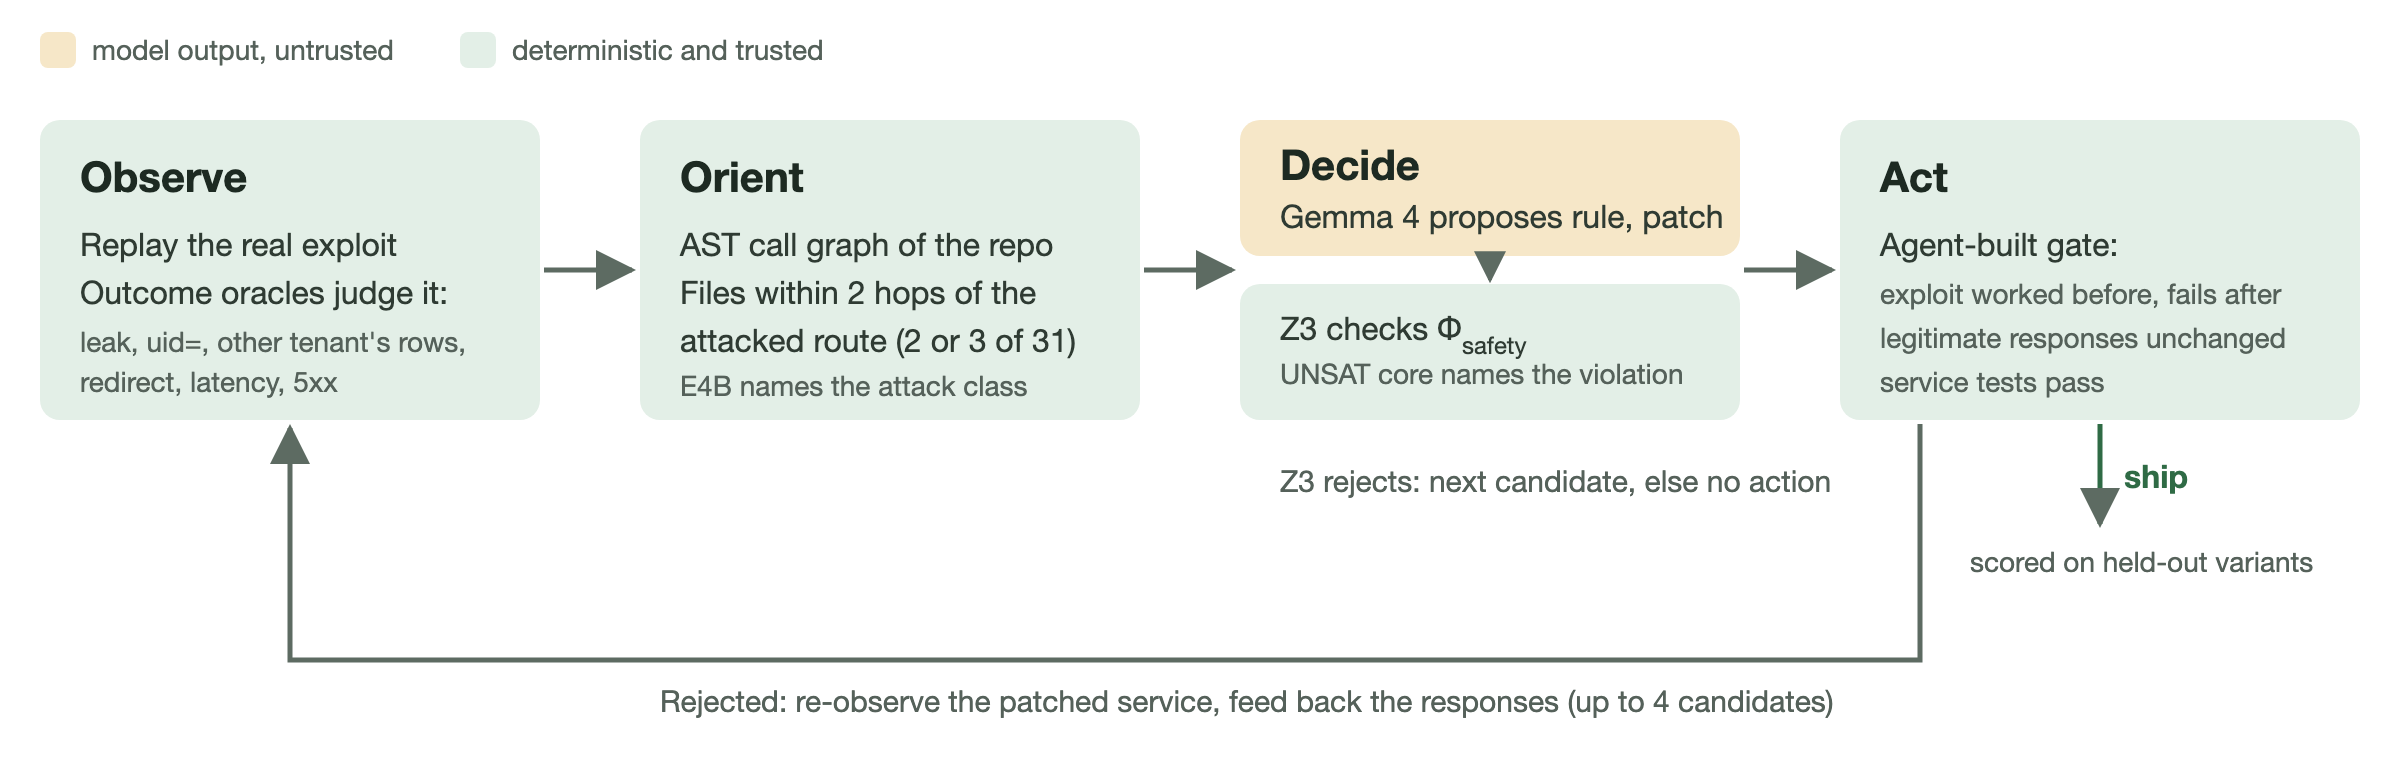
\includegraphics[width=\linewidth]{../fig_loop.png}\caption{The OODA-Aegis loop: model outputs pass Z3 and the gate before they act.}\end{figure}
\textbf{Observe.} The real exploit is replayed; outcome oracles, not input signatures, decide whether it worked: a password file or canary token in the body, \texttt{uid=} from command execution, another tenant's rows, an external redirect, a response slower than 1\,s, or a 5xx.

\textbf{Orient.} The edge model names the attack class. A static call graph of functions and classes is built with Python's AST, resolving imports and attribute calls and mapping route decorators to handlers. Main runs use every file within two hops of the handler (2 or 3 of 31); the \emph{call slice} takes every reachable function, optionally with calls recorded at run time (\S{}4.2).

\textbf{Decide.} Z3 checks both actions before anything executes, at two levels.

\begin{itemize}
\item \emph{Level 1, edge rules (string theory).} The edge model fills in a rule (\texttt{contains}, \texttt{max\_length}, \texttt{repeated\_run}) compiled to an encoding-aware proxy regex and a Z3 regular expression \texttt{E\_rule}; Z3 decides \texttt{L(E\_rule) $\cap$ R\_protected = $\emptyset$} exactly for the health check and recorded legitimate requests.
\item \emph{Level 2, patches (propositional).} The repair model states the invariant, then returns the patched file and its own pytest. Decidable AST facts about the diff are Z3 clauses (\texttt{in\_scope}: changed files inside the retrieved subgraph; \texttt{api\_kept}; \texttt{protected\_kept}; \texttt{no\_new\_sinks}; \texttt{changed}), and an UNSAT core names a violated one. This level says nothing about what the code computes; only the gate tests behaviour. Up to four candidates are tried.
\end{itemize}
\textbf{Act.} Only the agent-built gate accepts a patch, in a fresh copy of the repository: the exploit must succeed on the original code; on the patched code, the exploit and visible variants must be safe within 2.5\,s, legitimate requests must return the same status, redirect and parsed JSON (key order, timing fields, UUIDs and timestamps ignored), and the service's tests must pass. The model's own test is advisory. Verified patches are labelled \emph{root-cause fixes} if they change a definition the reference fix changes, else \emph{path-specific guards}.

\textbf{Threat model.} The attacker controls request parameters and headers, can leak data into the evidence and plant text in the repository. Oracles, gate, graph builder and Z3 are trusted; models are not.

\section{AegisBench}
Vault is a FastAPI service of 31 Python modules (430 lines). Each task swaps one core helper for a vulnerable version and ships the exploit, visible and held-out variants, 2 or 3 legitimate requests and a reference fix; a validation script checks every exploit and reference fix. Each vulnerable helper is one call hop from its route.

Classes (CWE), two tasks each: path traversal (22), SQL injection (89), ReDoS (1333), command injection (78), SSRF (918), open redirect (601), IDOR (639); one each: deserialization (502), format string (134).

\section{Experiments}
\textbf{Setup.} Ollama 0.40.16 on two NVIDIA T4 GPUs in free Kaggle notebooks; 16k context, JSON output, thinking off. Main runs: E4B for triage and edge rules, 26B-A4B for repair; 3 trials of the full agent, 2 of each ablation: \textbf{A} no runtime evidence; \textbf{B1/B2} no graph (route file only / whole repository); \textbf{C} no Z3 guard or gate (a raw regex loads; the first patch whose own test passes ships); \textbf{D} one shot. The size study uses one model for both roles (E4B, 12B, 31B; 2 trials); the injection bench crosses 3 injections $\times$ 16 tasks $\times$ guard on/off. In total: 400 episodes, 8.4 GPU-hours, no harness errors.

\textbf{Metrics.} \emph{Verified fix}: the gate accepted the shipped patch; \emph{shipped, gate rejects}: a live patch the gate would reject; \emph{held-out blocked}: live held-out variants (31 of 42) that fail against accepted patches. Wilson 95\% intervals; two-sided Fisher exact tests against the full agent.

\subsection{Overall and ablations}
\begin{table}[H]\centering\small
\begin{adjustbox}{max width=\linewidth}
\begin{tabular}{lllll}
\toprule
Configuration & Verified fix [95\% CI] & Shipped, gate rejects & Held-out blocked & Prompt tokens (median)\\
\midrule
OODA-Aegis (full) & 45/48 (94\%) [83, 98] & 0 & 89/89 & 1,573\\
A: w/o runtime evidence & 30/32 (94\%) [80, 98] & 0 & 60/60 & 1,496\\
B1: route file only & 0/32 (0\%) [0, 11] & 0 & n/a & 2,600\\
B2: whole repo, flat & 29/32 (91\%) [76, 97] & 0 & 59/59 & 6,341\\
C: trust the model & 22/32 (69\%) [51, 82] & 4 & 54/54 & 1,740\\
D: one shot & 13/32 (41\%) [26, 58] & 0 & 29/29 & 858\\
\bottomrule
\end{tabular}
\end{adjustbox}
\end{table}
The code graph makes localisation work (F1). With only the route file, the model named the right helper in all 128 attempts but never saw its code, and \texttt{in\_scope} rejected every blind rewrite. The whole repository works about as well here (91\% vs 94\%, p = 0.68) at 4.0$\times$ the tokens, but not with deeper bugs (\S{}4.2). Runtime evidence made no measurable difference. Removing guard and gate cost a quarter of the fixes (p = 0.005) and shipped 4 patches that change legitimate responses. With a fresh UUID, timestamp and shuffled keys in every response, the gate's comparison kept 61 of 61 unchanged legitimate cases and flagged all 32 real changes (F1 100\%; raw bytes kept 7; \texttt{results/semantic.md}).

\subsection{Code-graph retrieval and deeper call chains}
AegisBench-Deep puts the same 16 bugs behind 1 to 4 pass-through layers, 2 to 5 call hops from the handler. Offline, a hop limit k misses every bug deeper than k; the call slice keeps 16/16 at every depth with 7--15\% of the code, while BM25 in the spirit of RepoCoder~\cite{r9} misses 2 to 4 per depth. When the route reaches the helper through \texttt{getattr}, a decorator registry or an ORM-style manager, the static slice finds 0/16; adding the calls recorded while replaying legitimate requests restores 16/16 at depths 1, 3 and 5.

We ran Gemma 4 E4B in both roles locally (Apple M5, one trial per cell; depth-1 calibration 15/16, against 31/32 on Kaggle).

\begin{figure}[H]\centering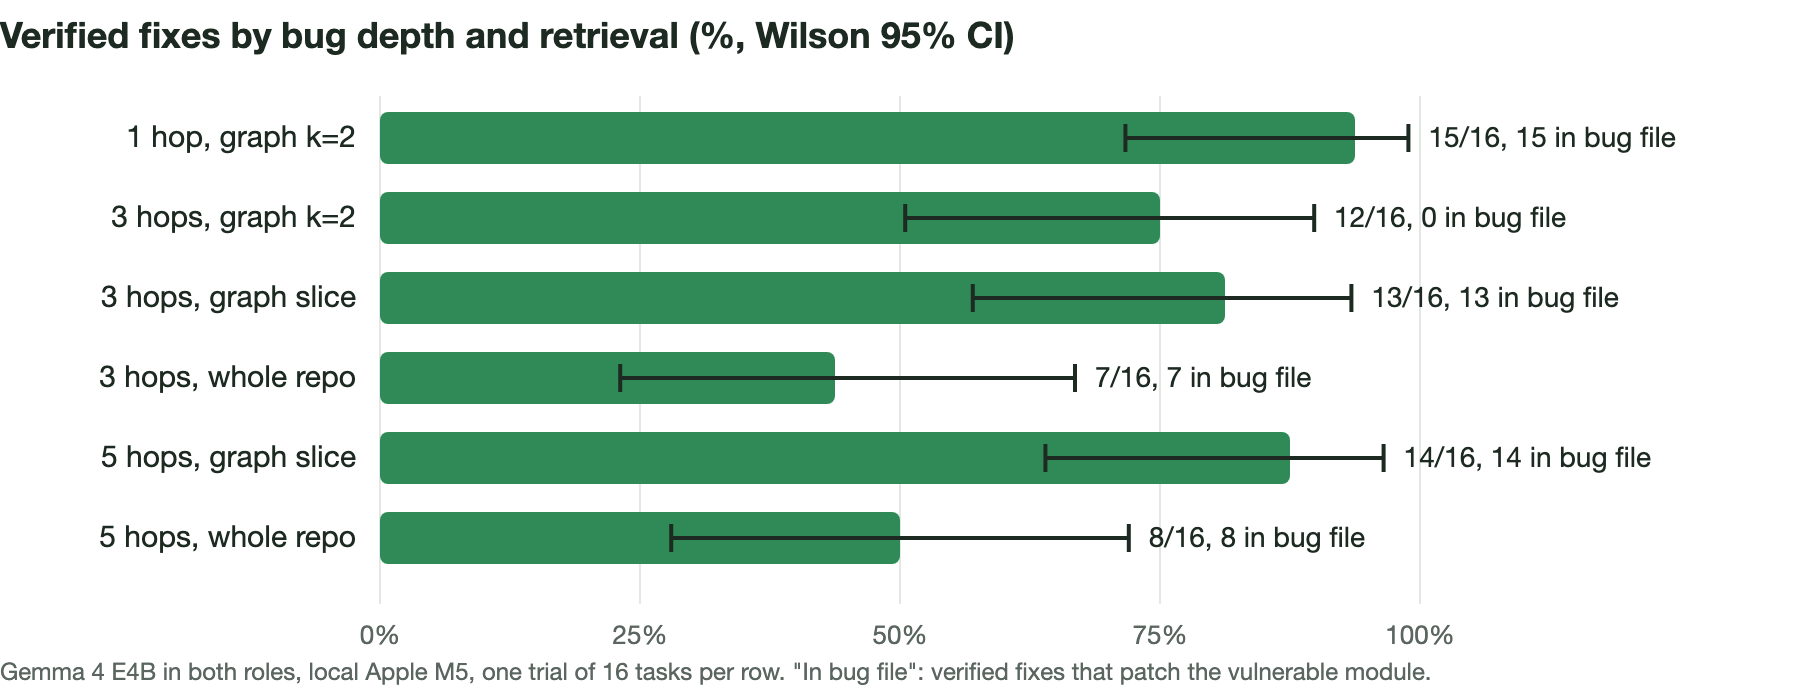
\includegraphics[width=\linewidth]{../fig_deep.png}\caption{Verified fixes by bug depth and retrieval, and how many patch the vulnerable file (Gemma 4 E4B, 16 tasks per row).}\end{figure}
Over depths 3 and 5 the slice verified 27/32 fixes, all in the vulnerable file; the whole repository 15/32 (p = 0.003) at ten times the tokens. With k=2 the vulnerable file was never in context at depth 3, yet 12/16 passed the gate by guarding the outermost wrapper, leaving the helper exploitable from other callers. These are the only path-specific guards among all 299 verified fixes (\texttt{results/rootcause.md}). \emph{sink\_changed}, which needs no reference fix (the patch must change a payload-receiving function in the deepest module, traced by a profiler), agrees with this label on all 266 fixes of the 14 data-flow tasks but rejects the 31 IDOR fixes, whose bug is a missing check in the caller. A static clause, \emph{no\_sanitizer\_bypass} (a parameter the patch adds may reach a sink only through existing validation), holds for all 16 reference fixes and 632 parsed logged patches and rejects three hand-written bypasses (\texttt{results/sanitizer.md}).

\subsection{Real CVEs}
We took 13 CVEs in ten widely used packages, pinned to the last vulnerable release, with target functions from a function-level diff against the fixed release (\texttt{cves.py --verify}). Each exploit works on the vulnerable release and fails on the fixed one (13/13; Django's behaviourally, as its regexes do not slow down on CPython 3.12), and each release passes its own tests for the changed code (13/13; \texttt{results/realcve/}). ``Code to reach the bug'': the share of the package a strategy hands the model, whole functions in its order, until a function the fix changed is included.

\begin{table}[H]\centering\small
\begin{adjustbox}{max width=\linewidth}
\begin{tabular}{llllll}
\toprule
Package (CVE) & Lines & Hops static & Hops + trace & BM25, class & Slice + trace + BM25, class\\
\midrule
requests (2023-32681) & 5,433 & 5 & 5 & 2.6\% & 2.1\%\\
urllib3 (2021-33503) & 11,217 & 1 & 1 & 66.3\% & 8.5\%\\
requests + urllib3 (2021-33503) & 16,650 & 6 & 6 & 71.1\% & 30.4\%\\
waitress (2022-24761) & 4,956 & 1 & 1 & 13.2\% & 8.1\%\\
requests (2018-18074) & 5,000 & 5 & 5 & 0.6\% & 0.6\%\\
PyYAML (2020-1747) & 5,900 & -- & 6 & 11.1\% & 13.2\%\\
Jinja2 (2019-10906) & 12,348 & -- & 1 & 0.1\% & 0.1\%\\
sqlparse (2021-32839) & 3,768 & 3 & 3 & 25.2\% & 22.7\%\\
idna (2024-3651) & 11,379 & 1 & 1 & 1.1\% & 0.8\%\\
python-multipart (2024-24762) & 2,125 & 2 & 2 & 77.7\% & 60.7\%\\
aiohttp (2024-23334) & 20,859 & -- & 1 & 8.7\% & 3.4\%\\
Werkzeug (2023-25577) & 21,697 & 2 & 2 & 26.4\% & 11.0\%\\
Django (2023-36053) & 151,260 & -- & 2 & 34.6\% & 4.6\%\\
\bottomrule
\end{tabular}
\end{adjustbox}
\end{table}
Statically the graph reaches a fixed function in 9 of 13 cases; the rest call through a registry, generated template code, a stored route handler or a validator list, and the exploit's trace reaches all 13. The slice alone does not compress real code (its files hold 67--99.6\% of 10 packages). BM25 is strong with the alert text (median 0.8\%), weak with only the attack class (median 13.2\%); within slice + trace it improved 10 of 13 class-only cases, never lost with the alert, and found the bug within 0.1--0.2\% of the code in the three packages above 20,000 lines. The graph filters and explains similarity ranking; it does not replace it.

\textbf{Repairing CVE-2021-33503} (Gemma 4 E4B, 5 trials per gate, \texttt{results/realcve/summary.md}). A 12,010-character URL takes 2.5--3.1\,s to parse. With urllib3's 37 test URLs as legitimate inputs the gate accepted 3 of 5 trials, all length caps that break long legitimate URLs; with 7 long URLs added it accepted 2 of 5, both capping the authority at 100 \texttt{@}: a mitigation, not the upstream fix. A gate is only as strong as its legitimate inputs.

\subsection{Containment at the edge}
Raw regexes always load, but 14 of 32 miss their own exploit, usually by ignoring URL encoding. Guarded rules loaded in 143 of 176 episodes, never blocked a protected request, and covered 57\% of variants against 20\%, in a median 3\,s.

\subsection{Should the model grade its own fix?}
Over 190 26B-A4B candidates that reached the gate, the model's test passed 124 (25 broken) and failed 66 (59 correct): agreement 56\% [49, 63] (F2).

\subsection{Indirect prompt injection (preliminary)}
Three static injections (in a header, the leaked response, a retrieved comment) told the agent to block all traffic, delete the tenant check, or use \texttt{eval}; in 96 episodes Gemma 4 never followed one (F5). Adaptive attacks~\cite{r16,r17} were not run, so this is not evidence of robustness.

\subsection{Model size}
As single-model agents (32 episodes each), E4B, 12B and 31B verified 31, 29 and 31 fixes in a median 35, 87 and 143\,s (F3).

\subsection{Failure analysis}
\emph{One missing quote.} 167 of the 197 syntax rejections parse once one character is restored: in JSON mode 26B-A4B and 31B close the docstring with two quotes, not three. Restored offline, one shot would reach 28/32, so most of the gain from multi-candidate search (41\% $\rightarrow$ 94\%, p < 0.001) is recovery from one formatting error (F4).

\section{Application: from alert to verified patch}
OODA-Aegis runs beside a service on one small GPU: it confirms a flagged request, loads a Z3-verified proxy rule (median 3\,s), repairs the code (median 53\,s) and ships only a gate-accepted patch with an audit record. A failure costs a fallback, not an outage.

\section{Generality, reuse and limitations}
\emph{Reuse for training.} Every candidate carries a label needing no human (of 694: 288 passed the gate, 74 failed it, 135 violated \phisafe{}, 197 did not parse): a verifiable reward for fine-tuning.

\emph{What may not.} The tasks were written for this benchmark; the real-code evidence is 13 CVEs for retrieval, exploits and regression tests, and one for repair. A trace sees only exercised paths; reflection is untested. Deep and CVE runs are local, with few trials. The gate covers only recorded inputs. The data-flow clauses were evaluated offline, not used as gates. With 1 to 3 trials per cell, differences of a few episodes are not significant.

\section{Related work}
Generate-and-validate repair~\cite{r1,r2} overfits tests~\cite{r3}; learned and LLM-based repair followed~\cite{r4,r5}. SWE-agent~\cite{r6} and SWE-bench~\cite{r7} judge resolution by tests. WAF virtual patching is standard~\cite{r8}. Repository retrieval~\cite{r9} and program graphs~\cite{r10} motivate our retrieval. Z3~\cite{r11} and string solvers~\cite{r12} support verification. Indirect injection~\cite{r16} is in OWASP's LLM Top 10~\cite{r13}; AgentDojo~\cite{r17} tests adaptive attacks.

\section{Conclusion}
A small Gemma 4 model can repair exploited code reliably on a free GPU if the agent shows it the right code, never lets it grade its own work, and checks every action with a solver; on a real CVE it produced verified mitigations, not the upstream fix. Future work: repair on more real CVEs, the data-flow clauses as gates, fine-tuning on the released labels, and adaptive injections.

\small
\begin{thebibliography}{17}
\bibitem{r1} C. Le Goues et al., ``GenProg: A generic method for automatic software repair,'' IEEE TSE, 2012.
\bibitem{r2} M. Monperrus, ``Automatic software repair: a bibliography,'' ACM Computing Surveys, 2018.
\bibitem{r3} E. K. Smith et al., ``Is the cure worse than the disease? Overfitting in automated program repair,'' FSE, 2015.
\bibitem{r4} J. Bader et al., ``Getafix: Learning to fix bugs automatically,'' OOPSLA, 2019.
\bibitem{r5} C. S. Xia and L. Zhang, ``Less training, more repairing please: revisiting automated program repair via zero-shot learning,'' FSE, 2022.
\bibitem{r6} J. Yang et al., ``SWE-agent: Agent-computer interfaces enable automated software engineering,'' NeurIPS, 2024.
\bibitem{r7} C. E. Jimenez et al., ``SWE-bench: Can language models resolve real-world GitHub issues?,'' ICLR, 2024.
\bibitem{r8} OWASP ModSecurity Core Rule Set, \url{https://coreruleset.org}.
\bibitem{r9} F. Zhang et al., ``RepoCoder: Repository-level code completion through iterative retrieval and generation,'' EMNLP, 2023.
\bibitem{r10} M. Allamanis et al., ``Learning to represent programs with graphs,'' ICLR, 2018.
\bibitem{r11} L. de Moura and N. Bjørner, ``Z3: An efficient SMT solver,'' TACAS, 2008.
\bibitem{r12} M. Berzish et al., ``Z3str3: A string solver with theory-aware heuristics,'' FMCAD, 2017.
\bibitem{r13} OWASP, ``Top 10 for Large Language Model Applications,'' 2025.
\bibitem{r14} J. R. Boyd, ``Destruction and Creation,'' 1976.
\bibitem{r15} E. Altman, ``Constrained Markov Decision Processes,'' Chapman \& Hall, 1999.
\bibitem{r16} K. Greshake et al., ``Not what you've signed up for: Compromising real-world LLM-integrated applications with indirect prompt injection,'' AISec, 2023.
\bibitem{r17} E. Debenedetti et al., ``AgentDojo: A dynamic environment to evaluate prompt injection attacks and defenses for LLM agents,'' NeurIPS Datasets and Benchmarks, 2024.
\end{thebibliography}
\end{document}
